\documentclass[12pt]{article}

\usepackage[margin=1in]{geometry}
\usepackage{booktabs}
\usepackage{longtable}
\usepackage{amsmath}
\usepackage{graphicx}
\usepackage{hyperref}
\usepackage{listings}
\usepackage{placeins}

\hypersetup{hidelinks}

\lstset{
  basicstyle=\small\ttfamily,
  columns=fullflexible,
  breaklines=true,
  frame=single
}

\renewcommand{\thesection}{S\arabic{section}}
\renewcommand{\thetable}{S\arabic{table}}
\renewcommand{\thefigure}{S\arabic{figure}}

\title{Supporting Information for\\
Algorithmic Construction and Exploitation of Topology-Constrained Refinement Models for Semiexperimental Equilibrium Structures}
\author{Vincenzo Barone}
\date{}

\begin{document}
\maketitle

\section{Global Benchmark Diagnostics}

Tables~\ref{tab:benchmark-summary} and~\ref{tab:planar-pair-diagnostics}
collect the numerical values underlying the graphical benchmark summaries in
the main text. A complete representative command, Cartesian and isotopologue
input, output manifest, and final diagnostic excerpt are given in
Section~\ref{sec:si-input-output}. The standalone source, runnable examples,
benchmark inputs, and machine-readable validation data are publicly available
in the revision-pinned MORPHEUS repository at
\url{https://github.com/yogibubu/morpheus}.

% Generated by `python -m matrix semiexp-benchmark --paper`.
\begin{table*}
\caption{One-page audit of the representative \texttt{MORPHEUS}
semiexperimental refinements. ``Model'' is the working-coordinate model used
for the main row. ``Fit'' gives the independent rotational components entering
the normal equations; for moment-based fits, $AB$ denotes $(I_a,I_b)$. ``GIC/A''
gives the algorithmically generated non-redundant coordinate count and the
totally symmetric active count before constraint projection. ``Eff./rank''
gives the independent variables after primitive-constraint projection and the
final numerical rank. Rotational residuals are RMS/maximum absolute values in
MHz over all reported diagnostic constants.}
\label{tab:benchmark-summary}
\scriptsize
\setlength{\tabcolsep}{2.0pt}
\begin{tabular}{@{}llclrcclcl@{}}
\toprule
System & PG & Model & Fit & Iso. & GIC/A & Eff./rank & Constraints & Steps & RMS/max \\
\midrule
Glycolaldehyde & C$_s$ & GIC & ABC & 10 & 18/12 & 12/12 & none & 3/0; min & 0.5640/1.7961 \\
Cyclopentadiene & C$_{2v}$ & Cart. & ABC & 14 & 27/10 & 10/10 & none & 10/0; min & 0.0635/0.2289 \\
Nitrobenzene & C$_{2v}$ & GIC & AB & 9 & 36/13 & 13/13 & 8 primitive & 4/0; pos. & 0.1480/0.2605 \\
p-EBN & C$_{2v}$ & GIC & AB & 11 & 39/14 & 6/6 & 22 frozen & 4/20; min & 0.1190/0.5674 \\
Azulene & C$_{2v}$ & GIC & AB & 12 & 48/17 & 10/10 & 8 primitive & 8/28; min & 0.0731/0.2900 \\
Norcamphor & C$_1$ & GIC & ABC & 9 & 48/48 & 18/18 & 30 H + 58 pred. & 12/7; min & 0.0941/0.2629 \\
Glycine I & C$_s$ & GIC & ABC & 5 & 24/15 & 11/11 & 4 function & 3/17; min & 0.0269/0.0570 \\
Glycine II & C$_1$ & GIC & ABC & 10 & 24/24 & 19/19 & 5 function & 26/8; min & 0.2491/0.6707 \\
\bottomrule
\end{tabular}
\end{table*}


% Generated by `python -m matrix semiexp-benchmark --paper`.
\begin{table*}
\caption{Planar-component diagnostics for the planar benchmarks. Only two
principal moments are independent for a planar molecule; the selected pair
marked by an asterisk is used in the normal equations, while all three
rotational constants are recomputed after convergence. The residuals are
RMS/maximum absolute MHz values over the complete diagnostic $A$, $B$, and $C$
constant set.}
\label{tab:planar-pair-diagnostics}
\scriptsize
\setlength{\tabcolsep}{4pt}
\begin{tabular}{@{}lclrrl@{}}
\toprule
System & Pair & Fitted moments & Rank & Cond. & Diagnostic RMS/max \\
\midrule
Nitrobenzene & AB$^\ast$ & $(I_a,I_b)$ & 13 & 27464.4 & 0.1480/0.2605 \\
Nitrobenzene & AC & $(I_a,I_c)$ & 13 & 56007.7 & 0.2593/0.4597 \\
Nitrobenzene & BC & $(I_b,I_c)$ & 13 & 10623.3 & 2.4602/4.3693 \\
Azulene & AB$^\ast$ & $(I_a,I_b)$ & 10 & 956.7 & 0.0731/0.2900 \\
Azulene & AC & $(I_a,I_c)$ & 10 & 1780.0 & 0.1086/0.4222 \\
Azulene & BC & $(I_b,I_c)$ & 10 & 950.2 & 0.3232/0.7541 \\
\bottomrule
\end{tabular}
\end{table*}


\section{Atom Numbering Used in the Tables}

Figure~\ref{fig:si-atom-numbering} gives the atom numbering used with the
structural tables and diagnostic comparisons. The same Cartesian numbering is
used by the topology perception, coordinate generation, and least-squares
reporting steps. The p-EBN structure is included as a legacy MSR-import
companion case for numbering consistency. For camphor, the atom numbering is
defined by the archived Cartesian input and by the full parameter tables in
Section~\ref{sec:si-camphor}.

\begin{figure}
\centering
\begin{minipage}{0.24\linewidth}
\centering
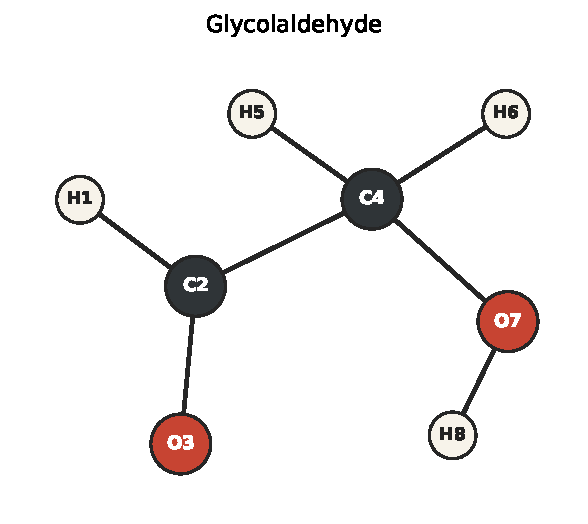
\includegraphics[width=\linewidth]{figures/glycolaldehyde_numbering.pdf}\\[-0.4em]
\end{minipage}
\begin{minipage}{0.24\linewidth}
\centering
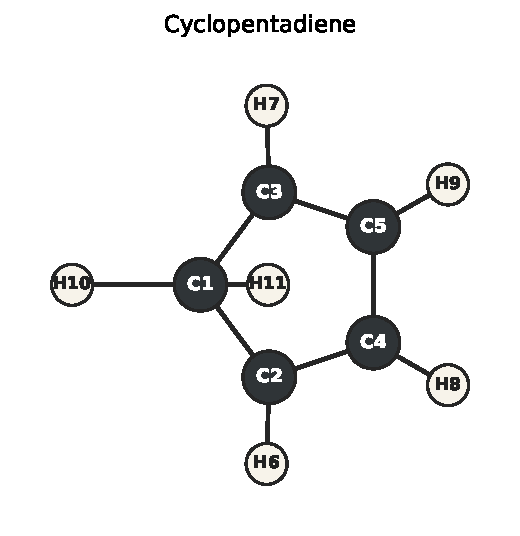
\includegraphics[width=\linewidth]{figures/cyclopentadiene_numbering.pdf}\\[-0.4em]
\end{minipage}
\begin{minipage}{0.24\linewidth}
\centering
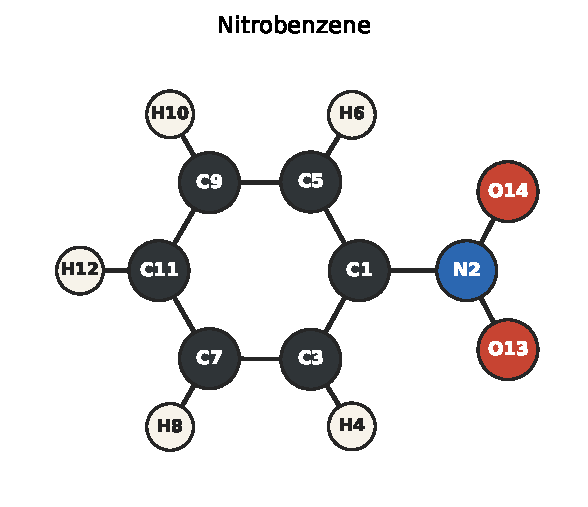
\includegraphics[width=\linewidth]{figures/nitrobenzene_numbering.pdf}\\[-0.4em]
\end{minipage}
\begin{minipage}{0.24\linewidth}
\centering
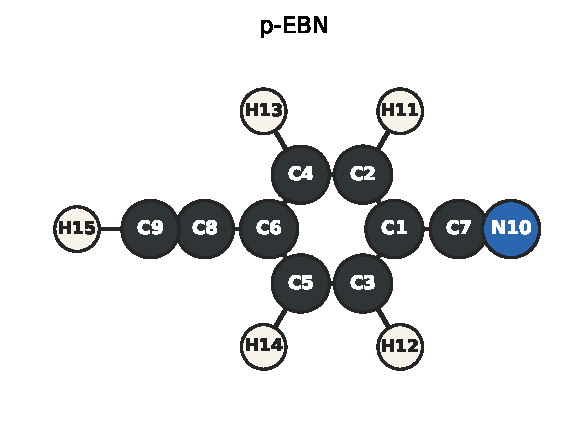
\includegraphics[width=\linewidth]{figures/p-EBN_numbering.pdf}\\[-0.4em]
\end{minipage}

\vspace{0.5em}

\begin{minipage}{0.24\linewidth}
\centering
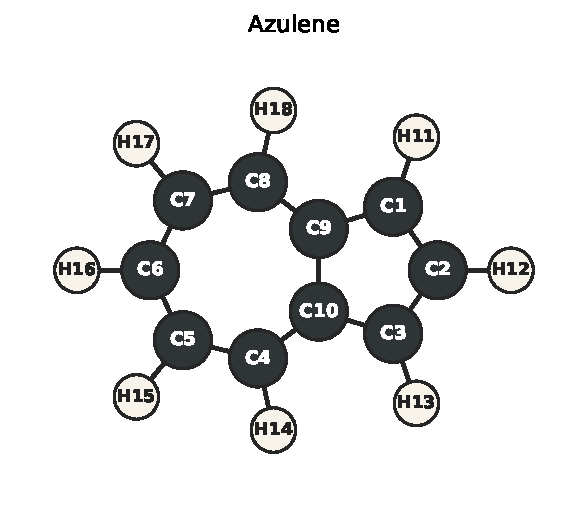
\includegraphics[width=\linewidth]{figures/azulene_numbering.pdf}\\[-0.4em]
\end{minipage}
\begin{minipage}{0.24\linewidth}
\centering
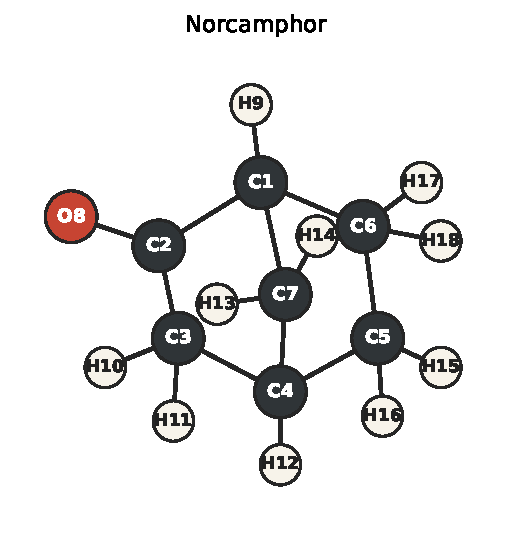
\includegraphics[width=\linewidth]{figures/norcamphor_numbering.pdf}\\[-0.4em]
\end{minipage}
\begin{minipage}{0.24\linewidth}
\centering
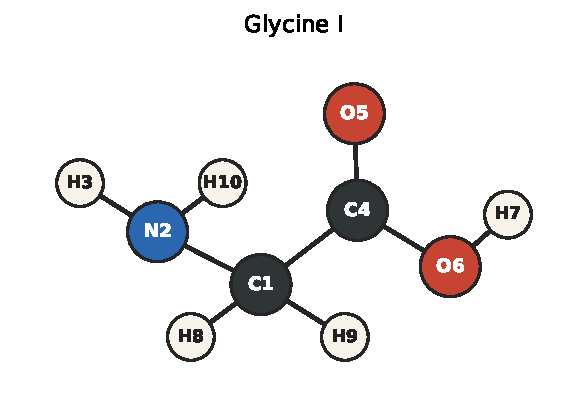
\includegraphics[width=\linewidth]{figures/glycine_I_numbering.pdf}\\[-0.4em]
\end{minipage}
\begin{minipage}{0.24\linewidth}
\centering
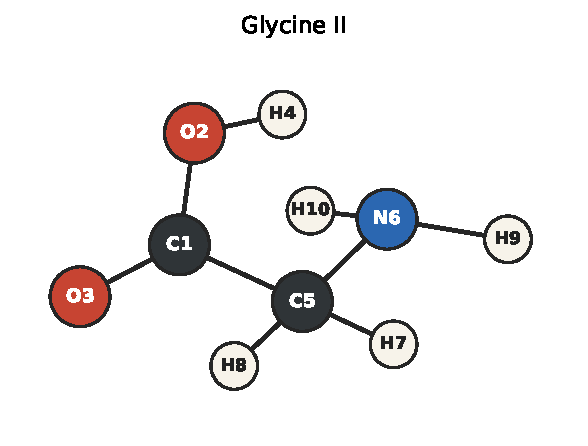
\includegraphics[width=\linewidth]{figures/glycine_II_numbering.pdf}\\[-0.4em]
\end{minipage}

\vspace{0.5em}

\begin{minipage}{0.24\linewidth}
\centering
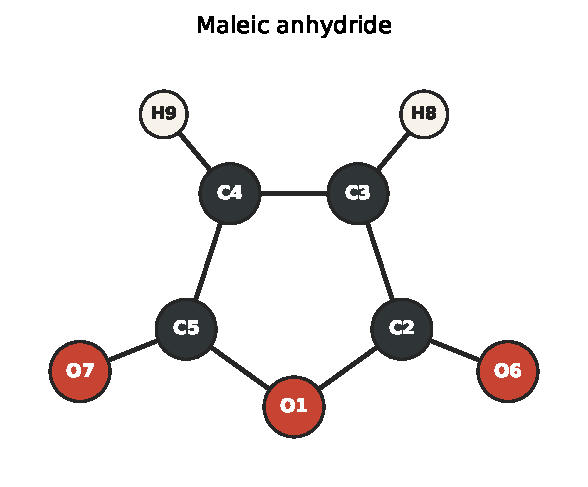
\includegraphics[width=\linewidth]{figures/maleic_anhydride_numbering.pdf}\\[-0.4em]
\end{minipage}
\begin{minipage}{0.24\linewidth}
\centering
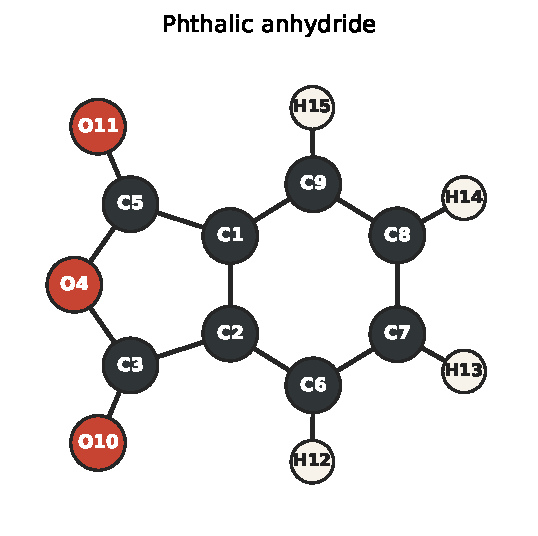
\includegraphics[width=\linewidth]{figures/phthalic_anhydride_numbering.pdf}\\[-0.4em]
\end{minipage}
\begin{minipage}{0.24\linewidth}
\centering
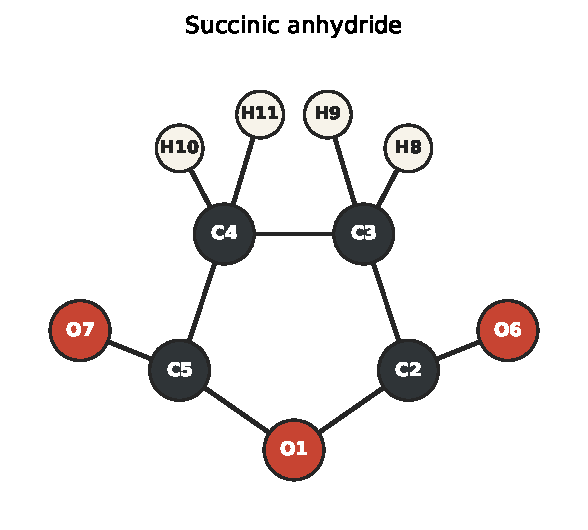
\includegraphics[width=\linewidth]{figures/succinic_anhydride_numbering.pdf}\\[-0.4em]
\end{minipage}
\begin{minipage}{0.24\linewidth}
\centering
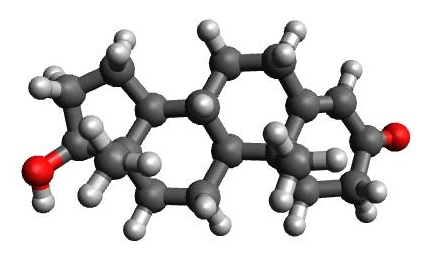
\includegraphics[width=\linewidth]{figures/testosterone_qc_cropped.jpg}\\[-0.4em]
\end{minipage}
\caption{Atom numbering used for the benchmark and companion structures:
glycolaldehyde, cyclopentadiene, nitrobenzene, p-EBN, azulene, norcamphor,
glycine I, glycine II, and the maleic, phthalic, and succinic anhydride
series. Testosterone is included as the 49-atom fused-ring scale check.}
\label{fig:si-atom-numbering}
\end{figure}

\begin{table}
\caption{Comparison of MORPHEUS working-coordinate models. ``Work.'' is the number
of non-redundant GICs or symmetry-adapted Cartesian vibrational directions,
``Sym.'' is the number of totally symmetric working coordinates before
primitive-constraint projection, and ``Eff.'' is the number of independent
least-squares variables after projection. Residuals are RMS/maximum absolute
values in MHz.}
\label{tab:si-coordinate-models}
\small
\begin{tabular}{llrrrrrl}
\toprule
System & Model & Work. & Sym. & Eff. & Rank & Cond. & Residuals \\
\midrule
Cyclopentadiene & GICs & 27 & 10 & 10 & 10 & 454.5 & 0.0635/0.2289 \\
Cyclopentadiene & Sym. Cart. & 27 & 10 & 10 & 10 & 635.4 & 0.0635/0.2289 \\
p-EBN & GICs & 39 & 14 & 6 & 6 & 2440.2 & 0.1190/0.5674 \\
Azulene & GICs & 48 & 17 & 10 & 10 & 956.7 & 0.0731/0.2900 \\
Azulene & Sym. Cart. & 48 & 17 & 10 & 10 & 744.8 & 0.0731/0.2900 \\
Norcamphor & GICs & 48 & 48 & 18 & 18 & 5199.2 & 0.0941/0.2629 \\
Norcamphor & Sym. Cart. & 48 & 48 & 18 & 18 & 4216.7 & 0.0941/0.2629 \\
Camphor & GICs & 75 & 75 & 75 & 75 & 71.3 & 0.0788/0.2839 \\
Camphor & Sym. Cart. & 75 & 75 & 75 & 75 & 23.5 & 0.0788/0.2839 \\
\bottomrule
\end{tabular}
\end{table}

The norcamphor rows use the standalone \texttt{xyzin} file archived in the
MORPHEUS norcamphor example directory.  That file contains the DPCS3 Cartesian
geometry, the experimental rotational constants from Table 3 of the
norcamphor rotational study, and the tabulated vibrational corrections.  The
reported run adds 58 Kraitchman-derived soft predicates with
$\sigma_R=0.003$~\AA{} and $\sigma_A=0.3^\circ$; the same predicate set gives
the same residual with GIC and symmetry-adapted Cartesian working coordinates.

The camphor rows report the accepted no-Kraitchman model described in
Section~\ref{sec:si-camphor}. The same BDPCS3-predicate model was replayed
with symmetry-adapted Cartesian working coordinates as a final-validation
check, not as a separate manually constructed refinement.

\section{Camphor Model-Validation Stress Test}
\label{sec:si-camphor}

The camphor data set is included to document the final validation layer rather
than to add another ordinary benchmark. The accepted model uses the BDPCS3
Cartesian geometry as the reference structure, 12 isotopologue records, the
three principal moments for each isotopologue, and 178 BDPCS3 soft predicates.
No hydrogen coordinate is fixed. C--H distances and hydrogen angles enter as
strict soft predicates from the BDPCS3 reference, whereas Kraitchman-derived
relations are retained only as diagnostics unless explicitly tested as
additional predicates. The files needed to regenerate the tables are archived
in \texttt{data/camphor}.

% Generated by scripts/generate_camphor_material.py.
\begin{center}
\refstepcounter{table}\label{tab:si-camphor-geometry-statistics}
\parbox{0.94\linewidth}{\small\raggedright Table~\thetable: Camphor accepted no-Kraitchman model. Signed shifts are final SE minus BDPCS3 initial values; propagated errors are standard errors from the final covariance.\par}
\smallskip
\footnotesize
\begin{tabular}{lrrrrr}
\toprule
Parameter set & Count & Mean shift & RMS shift & Max $|$shift$|$ & Mean/max error \\
\midrule
Bonds / m\AA{} & 28 & -0.011 & 0.314 & 0.832 & 2.819/3.000 \\
Angles / deg & 57 & -0.000 & 0.015 & 0.040 & 0.183/0.257 \\
Dihedrals / deg & 93 & 0.001 & 0.014 & 0.041 & 0.174/0.226 \\
\bottomrule
\end{tabular}
\end{center}


% Generated by scripts/generate_camphor_material.py.
\begin{center}
\refstepcounter{table}\label{tab:si-camphor-stability-controls}
\parbox{0.94\linewidth}{\small\raggedright Table~\thetable: Camphor stability controls. Geometry columns report maximum absolute final-minus-BDPCS3 deviations in the corresponding run.\par}
\smallskip
\scriptsize
\resizebox{\textwidth}{!}{%
\begin{tabular}{lrrrrrl}
\toprule
Model variant & RMS / MHz & Rank & Cond. & Max bond / m\AA{} & Max angle / deg & Outcome \\
\midrule
No-Kraitchman BDPCS3 predicates & 0.0788 & 75 & 71.3 & 0.832 & 0.040 & retained \\
Symmetry-Cartesian replay & 0.0788 & 75 & 23.5 & 0.832 & 0.040 & same model \\
All predicate errors x3 & 0.0727 & 75 & 112.5 & 0.834 & 0.045 & stable \\
BDPCS3 + broad Kraitchman & 0.0780 & 75 & 71.1 & 0.930 & 0.051 & not retained \\
BDPCS3 + tight Kraitchman & 0.0840 & 75 & 69.8 & 7.645 & 0.343 & rejected \\
No H predicates & 0.0629 & 36 & $\infty$ & 159.509 & 5.284 & rejected \\
Partial Kraitchman model & 0.2415 & 75 & 4.04e+04 & 90.580 & 6.224 & rejected \\
\bottomrule
\end{tabular}%
}
\end{center}


% Generated by scripts/generate_camphor_material.py.
\begin{center}
\refstepcounter{table}\label{tab:si-camphor-kraitchman}
\parbox{0.94\linewidth}{\small\raggedright Table~\thetable: Kraitchman-derived trial predicates for camphor compared with BDPCS3 reference parameters. Full CSV: \texttt{data/camphor/kraitchman\_predicate\_vs\_bdpcs3.csv}.\par}
\smallskip
\footnotesize
\begin{tabular}{lrrrl}
\toprule
Set & Count & RMS diff. & Max $|$diff.$|$ & Largest example \\
\midrule
Distances / m\AA{} & 28 & 38.352 & 92.760 & R(13,25) (-92.760) \\
Angles / deg & 57 & 2.740 & 6.188 & A(25,13,26) (6.188) \\
\bottomrule
\end{tabular}
\end{center}


The final geometry table shows that the accepted model is a small correction
to the BDPCS3 structure: the largest bond and valence-angle shifts are
0.832~m\AA{} and $0.040^\circ$, respectively. The validation controls show why
the lower residual obtained when hydrogen predicates are removed is not a
better model: the rank is lost and the geometry moves by chemically
unacceptable amounts. Similarly, tight Kraitchman-derived predicates distort
the structure, while broad Kraitchman predicates are harmless but add no
useful information beyond the validated BDPCS3-predicate model. The compact
final-validation summary is reported in the main text; the full
leave-predicate-group-out, sigma-scan, robust-loss, and multistart run table is
archived as \texttt{data/camphor/camphor\_final\_validation\_runs.csv}.

\clearpage

\begin{table}
\caption{Legacy MSR/MSROT compatibility checks. For systems where manually
constructed legacy inputs are available with the same active information,
MORPHEUS reproduces the MSR/MSROT numerical model while generating the
coordinate basis and projection operators automatically. Residuals are
RMS/maximum absolute rotational residuals in MHz.}
\label{tab:si-msrot-checks}
\footnotesize
\begin{tabular}{llll}
\toprule
System & Legacy comparison & Active information & Residuals \\
\midrule
Cyclopentadiene & MSR/MSROT input & same active GIC space & 0.0635/0.2289 \\
Azulene & MSR-comparable subset & fixed C--H data; $AB$ pair & 0.0731/0.2900 \\
\bottomrule
\end{tabular}
\end{table}

These checks are not additional fitted models: they verify that, at fixed
active coordinates and fixed experimental input, the algorithmically generated
MORPHEUS model reaches the same numerical result as the corresponding
manually prepared MSR/MSROT setup.

\section{\texorpdfstring{Glycine I C$_s$ Constraint Benchmark}{Glycine I Cs Constraint Benchmark}}

Table~\ref{tab:si-glycine-I-rotconstants} reports the Gly-I benchmark run from
the QC reference Cartesian geometry with no stored structural constraints. The fit uses
moments of inertia as observables and all three rotational components because
the C$_s$ structure is not a planar rotor in the inertial sense: the two
methylene and two amino hydrogens lie outside the heavy-atom plane. The
ground-state constants and statistical weights are from Godfrey and Brown,
J. Am. Chem. Soc. 117, 2019-2023 (1995), Table 1. The corrected constants are
$B_e=B_0+\Delta B_\mathrm{vib}$ with the Gly-Ip zero-point corrections of
Kasalov{\'a} et al. The MORPHEUS advisor generated the following four hard
constraints from the QC reference geometry and isotope-availability pattern:
\begin{verbatim}
HNH(Frozen,Value=105.634453352622)=A(3,2,10)
NH2WAG(Frozen,Value=55.901476176288)=U(2,10,3,1)
ROH(Frozen,Value=0.965159162788)=R(6,7)
ACOH(Frozen,Value=106.584216097335)=A(4,6,7)
\end{verbatim}
The numerical data entering the fit are collected in
Table~\ref{tab:si-glycine-I-inputdata} so that the corrected constants can be
reproduced without consulting the original tables.

\begin{longtable}{llrrrr}
\caption{Glycine I rotational input data. $B_0$, $\sigma(B_0)$, $\Delta B_\mathrm{vib}$, and $B_e=B_0+\Delta B_\mathrm{vib}$ are in MHz. The $^{13}$C(1) and $^{13}$C(2) labels of Godfrey and Brown correspond here to C13\_carboxyl and C13\_methylene, respectively.}\label{tab:si-glycine-I-inputdata}\\
\toprule
Isotopologue & Constant & $B_0$ & $\sigma(B_0)$ & $\Delta B_\mathrm{vib}$ & $B_e$ \\
\midrule
\endfirsthead
\toprule
Isotopologue & Constant & $B_0$ & $\sigma(B_0)$ & $\Delta B_\mathrm{vib}$ & $B_e$ \\
\midrule
\endhead
parent & A & 10341.5210 & 0.0890 & 78.6700 & 10420.1910 \\
parent & B & 3876.1785 & 0.0012 & 31.3000 & 3907.4785 \\
parent & C & 2912.3509 & 0.0010 & 22.3300 & 2934.6809 \\
C13\_carboxyl & A & 10340.9430 & 0.0290 & 77.8000 & 10418.7430 \\
C13\_carboxyl & B & 3869.1142 & 0.0057 & 30.9500 & 3900.0642 \\
C13\_carboxyl & C & 2908.3166 & 0.0026 & 22.0600 & 2930.3766 \\
C13\_methylene & A & 10227.0840 & 0.0880 & 76.7300 & 10303.8140 \\
C13\_methylene & B & 3859.0510 & 0.0210 & 30.9500 & 3890.0010 \\
C13\_methylene & C & 2893.5960 & 0.0200 & 21.9200 & 2915.5160 \\
CD2 & A & 9318.4520 & 0.0230 & 69.8400 & 9388.2920 \\
CD2 & B & 3799.2353 & 0.0023 & 31.2100 & 3830.4453 \\
CD2 & C & 2832.3222 & 0.0015 & 21.4800 & 2853.8022 \\
N15 & A & 10341.4500 & 0.1200 & 78.7600 & 10420.2100 \\
N15 & B & 3762.4570 & 0.0530 & 30.1300 & 3792.5870 \\
N15 & C & 2847.6390 & 0.0290 & 21.7100 & 2869.3490 \\
\bottomrule
\end{longtable}

\begin{longtable}{llrrr}
\caption{Complete rotational-constant comparison for glycine I. Corrected experimental constants, calculated constants, and differences are in MHz.}\label{tab:si-glycine-I-rotconstants}\\
\toprule
Isotopologue & Constant & Corrected exp. & Calculated & Difference \\
\midrule
\endfirsthead
\toprule
Isotopologue & Constant & Corrected exp. & Calculated & Difference \\
\midrule
\endhead
parent & A & 10420.1910 & 10420.2481 & -0.0570 \\
parent & B & 3907.4785 & 3907.4786 & -0.0001 \\
parent & C & 2934.6809 & 2934.6808 & +0.0001 \\
C13\_carboxyl & A & 10418.7430 & 10418.7403 & +0.0027 \\
C13\_carboxyl & B & 3900.0642 & 3900.0634 & +0.0008 \\
C13\_carboxyl & C & 2930.3766 & 2930.3769 & -0.0003 \\
C13\_methylene & A & 10303.8140 & 10303.7637 & +0.0503 \\
C13\_methylene & B & 3890.0010 & 3889.9809 & +0.0201 \\
C13\_methylene & C & 2915.5160 & 2915.5484 & -0.0324 \\
CD2 & A & 9388.2920 & 9388.2920 & +0.0000 \\
CD2 & B & 3830.4453 & 3830.4453 & -0.0000 \\
CD2 & C & 2853.8022 & 2853.8022 & -0.0000 \\
N15 & A & 10420.2100 & 10420.2444 & -0.0344 \\
N15 & B & 3792.5870 & 3792.5436 & +0.0434 \\
N15 & C & 2869.3490 & 2869.3715 & -0.0225 \\
\bottomrule
\end{longtable}

\begin{longtable}{llrr}
\caption{Selected primitive structural parameters for the glycine I C$_s$ benchmark with MORPHEUS-generated constraints. Bond lengths are in \AA; angles and dihedrals are in degrees.}\label{tab:si-glycine-I-geometry}\\
\toprule
Parameter & Description & Value & Std. error \\
\midrule
\endfirsthead
\toprule
Parameter & Description & Value & Std. error \\
\midrule
\endhead
R(1,2) & C--N & 1.44285 & 0.00076 \\
R(1,4) & C--C & 1.51134 & 0.00085 \\
R(1,8) & C--H & 1.09081 & 0.00021 \\
R(1,9) & C--H & 1.09081 & 0.00021 \\
R(2,3) & N--H & 1.00228 & 0.00011 \\
R(2,10) & N--H & 1.00228 & 0.00011 \\
R(4,5) & C--O & 1.20529 & 0.00184 \\
R(4,6) & C--O & 1.35001 & 0.00128 \\
R(6,7) & O--H & 0.96516 & 0.00000 \\
A(2,1,4) & N--C--C & 115.266 & 0.062 \\
A(8,1,9) & H--C--H & 105.923 & 0.031 \\
A(3,2,10) & H--N--H & 105.634 & 0.000 \\
A(1,4,5) & C--C--O & 125.338 & 0.095 \\
A(1,4,6) & C--C--O & 111.640 & 0.123 \\
A(5,4,6) & O--C--O & 123.022 & 0.060 \\
A(4,6,7) & C--O--H & 106.584 & 0.000 \\
D(2,1,4,5) & N--C--C--O & 180.000 & 0.000 \\
D(1,4,6,7) & C--C--O--H & 0.000 & 0.000 \\
D(8,1,4,5) & H--C--C--O & -56.781 & 0.030 \\
D(9,1,4,5) & H--C--C--O & 56.781 & 0.030 \\
\bottomrule
\end{longtable}

\section{Glycine II Functional-Constraint Benchmark}

Table~\ref{tab:si-glycine-rotconstants} reports the Gly-II advisor-constrained
benchmark discussed in the main text. The fit uses moments of inertia as
observables, but the diagnostic table is reported in MHz. The corrected
experimental constants are $B_e=B_0+\Delta B_\mathrm{vib}$ with the Gly-IIn
zero-point corrections. The Cartesian input does not store constraints; the
five functional constraints are generated by the MORPHEUS advisor from the QC
geometry and the isotopologue coverage.

\begin{longtable}{llrrr}
\caption{Complete rotational-constant comparison for glycine II. Corrected experimental constants, calculated constants, and differences are in MHz.}\label{tab:si-glycine-rotconstants}\\
\toprule
Isotopologue & Constant & Corrected exp. & Calculated & Difference \\
\midrule
\endfirsthead
\toprule
Isotopologue & Constant & Corrected exp. & Calculated & Difference \\
\midrule
\endhead
parent & A & 10195.5900 & 10196.2607 & -0.6707 \\
parent & B & 4105.3670 & 4105.3251 & 0.0419 \\
parent & C & 3039.8450 & 3039.8159 & 0.0291 \\
N15 & A & 10194.1150 & 10194.6721 & -0.5571 \\
N15 & B & 3994.8380 & 3994.8046 & 0.0334 \\
N15 & C & 2978.7993 & 2978.7971 & 0.0022 \\
C13\_methylene & A & 10060.9700 & 10061.6298 & -0.6598 \\
C13\_methylene & B & 4088.6720 & 4088.5073 & 0.1647 \\
C13\_methylene & C & 3018.8730 & 3018.8495 & 0.0235 \\
C13\_carboxyl & A & 10195.6980 & 10195.0945 & 0.6035 \\
C13\_carboxyl & B & 4093.0000 & 4093.1241 & -0.1241 \\
C13\_carboxyl & C & 3033.1070 & 3033.1532 & -0.0462 \\
O18\_carbonyl & A & 10064.2400 & 10063.7580 & 0.4820 \\
O18\_carbonyl & B & 3929.9160 & 3929.9078 & 0.0082 \\
O18\_carbonyl & C & 2931.7130 & 2931.8037 & -0.0907 \\
O18\_hydroxyl & A & 9580.9720 & 9580.9886 & -0.0166 \\
O18\_hydroxyl & B & 4090.8498 & 4090.8965 & -0.0467 \\
O18\_hydroxyl & C & 2975.1370 & 2975.1377 & -0.0007 \\
OD\_NH2 & A & 9792.2000 & 9792.2302 & -0.0302 \\
OD\_NH2 & B & 4096.1490 & 4096.1104 & 0.0386 \\
OD\_NH2 & C & 2998.1238 & 2998.0987 & 0.0251 \\
CD2 & A & 9145.3030 & 9145.3053 & -0.0023 \\
CD2 & B & 4020.3863 & 4020.3836 & 0.0027 \\
CD2 & C & 2947.9923 & 2947.9913 & 0.0010 \\
OH\_ND2 & A & 9927.6990 & 9927.6852 & 0.0138 \\
OH\_ND2 & B & 3716.3758 & 3716.3613 & 0.0145 \\
OH\_ND2 & C & 2841.7341 & 2841.7204 & 0.0137 \\
OD\_ND2 & A & 9542.6600 & 9542.6581 & 0.0019 \\
OD\_ND2 & B & 3710.5050 & 3710.5504 & -0.0454 \\
OD\_ND2 & C & 2806.0910 & 2806.1569 & -0.0659 \\
\bottomrule
\end{longtable}

\section{Cyclopentadiene Benchmark}

Table~\ref{tab:si-cyclopentadiene-rotconstants} reports the complete
comparison between corrected experimental rotational constants and constants
calculated from the final semiexperimental structure. The workflow uses
generalized internal coordinates (GICs) supplied by the companion SONIC
construction from the perceived primitive/B source, or symmetry-adapted Cartesian coordinates consumed by
\texttt{MORPHEUS}. The data set contains 14
isotopologues and all three principal rotational constants for each
isotopologue. The MORPHEUS refinement uses only a Cartesian representation of the
molecular structure, whereas the MSR refinement used manual Z-matrix
coordinates and constraints.

\begin{longtable}{llrrr}
\caption{Complete rotational-constant comparison for the cyclopentadiene benchmark derived from MSR data. Corrected experimental and calculated constants are in MHz.}\label{tab:si-cyclopentadiene-rotconstants}\\
\toprule
Isotopologue & Component & Corrected exp. & Calculated & Difference \\
\midrule
\endfirsthead
\toprule
Isotopologue & Component & Corrected exp. & Calculated & Difference \\
\midrule
\endhead
msr\_symm\_01 & A & 8489.154993 & 8489.232117 & -0.077124 \\
msr\_symm\_01 & B & 8292.100993 & 8292.093033 & 0.007960 \\
msr\_symm\_01 & C & 4305.664997 & 4305.658417 & 0.006580 \\
msr\_symm\_02 & A & 8292.098993 & 8292.093033 & 0.005960 \\
msr\_symm\_02 & B & 8280.278992 & 8280.319224 & -0.040231 \\
msr\_symm\_02 & C & 4251.270992 & 4251.257436 & 0.013556 \\
msr\_symm\_03 & A & 8482.790995 & 8482.866229 & -0.075234 \\
msr\_symm\_03 & B & 8105.052002 & 8105.082639 & -0.030637 \\
msr\_symm\_03 & C & 4253.082997 & 4253.084517 & -0.001520 \\
msr\_symm\_04 & A & 8408.381002 & 8408.358013 & 0.022989 \\
msr\_symm\_04 & B & 8172.557990 & 8172.606506 & -0.048516 \\
msr\_symm\_04 & C & 4252.643011 & 4252.628488 & 0.014523 \\
msr\_symm\_05 & A & 8408.381002 & 8408.358024 & 0.022978 \\
msr\_symm\_05 & B & 8172.557990 & 8172.606496 & -0.048506 \\
msr\_symm\_05 & C & 4252.643011 & 4252.628488 & 0.014523 \\
msr\_symm\_06 & A & 8195.611995 & 8195.593227 & 0.018768 \\
msr\_symm\_06 & B & 7918.397999 & 7918.289812 & 0.108187 \\
msr\_symm\_06 & C & 4178.352982 & 4178.398406 & -0.045424 \\
msr\_symm\_07 & A & 8195.611995 & 8195.612584 & -0.000589 \\
msr\_symm\_07 & B & 7918.397999 & 7918.308530 & 0.089469 \\
msr\_symm\_07 & C & 4178.352982 & 4178.398587 & -0.045604 \\
msr\_symm\_08 & A & 8477.175001 & 8477.228373 & -0.053372 \\
msr\_symm\_08 & B & 7650.516996 & 7650.483876 & 0.033120 \\
msr\_symm\_08 & C & 4123.171991 & 4123.147057 & 0.024934 \\
msr\_symm\_09 & A & 8477.175001 & 8477.228367 & -0.053366 \\
msr\_symm\_09 & B & 7650.516996 & 7650.483883 & 0.033113 \\
msr\_symm\_09 & C & 4123.171991 & 4123.147057 & 0.024933 \\
msr\_symm\_10 & A & 8371.829003 & 8371.953330 & -0.124328 \\
msr\_symm\_10 & B & 7735.107991 & 7735.111002 & -0.003010 \\
msr\_symm\_10 & C & 4122.272002 & 4122.241235 & 0.030767 \\
msr\_symm\_11 & A & 8371.829003 & 8371.953344 & -0.124341 \\
msr\_symm\_11 & B & 7735.107991 & 7735.110990 & -0.002998 \\
msr\_symm\_11 & C & 4122.272002 & 4122.241235 & 0.030767 \\
msr\_symm\_12 & A & 7057.547996 & 7057.656561 & -0.108565 \\
msr\_symm\_12 & B & 6730.362994 & 6730.334074 & 0.028920 \\
msr\_symm\_12 & C & 3555.255987 & 3555.260397 & -0.004410 \\
msr\_symm\_13 & A & 7057.547996 & 7057.672705 & -0.124709 \\
msr\_symm\_13 & B & 6730.362994 & 6730.349532 & 0.013462 \\
msr\_symm\_13 & C & 3555.255987 & 3555.260180 & -0.004193 \\
msr\_symm\_14 & A & 6656.949995 & 6656.991310 & -0.041315 \\
msr\_symm\_14 & B & 6653.764996 & 6653.536122 & 0.228874 \\
msr\_symm\_14 & C & 3469.286997 & 3469.303412 & -0.016415 \\
\bottomrule
\end{longtable}

\section{Nitrobenzene Planar Benchmark}

Nitrobenzene is a planar aromatic benchmark. The least-squares fit used the
independent $AB$ moment pair, corresponding to $(I_a,I_b)$, while the $C$
constants were recomputed from the optimized Cartesian geometry and retained as
diagnostic quantities. Table~\ref{tab:si-nitrobenzene-rotconstants} reports the
complete diagnostic comparison.

\begin{longtable}{llrrr}
\caption{Complete rotational-constant comparison for the nitrobenzene planar benchmark. Corrected experimental and calculated constants are in MHz. The fit used the independent $AB$ pair; the $C$ component is diagnostic.}\label{tab:si-nitrobenzene-rotconstants}\\
\toprule
Isotopologue & Component & Corrected exp. & Calculated & Difference \\
\midrule
\endfirsthead
\toprule
Isotopologue & Component & Corrected exp. & Calculated & Difference \\
\midrule
\endhead
parent & A & 3995.209000 & 3995.211821 & -0.002821 \\
parent & B & 1296.305300 & 1296.307106 & -0.001806 \\
parent & C & 979.000500 & 978.740045 & +0.260455 \\
N15 & A & 3995.193000 & 3995.211821 & -0.018821 \\
N15 & B & 1287.445000 & 1287.445036 & -0.000036 \\
N15 & C & 973.938200 & 973.679678 & +0.258522 \\
O18 & A & 3925.992000 & 3925.984021 & +0.007979 \\
O18 & B & 1264.689700 & 1264.689116 & +0.000584 \\
O18 & C & 956.803400 & 956.552095 & +0.251305 \\
6C13 & A & 3995.172000 & 3995.211821 & -0.039821 \\
6C13 & B & 1274.812600 & 1274.812638 & -0.000038 \\
6C13 & C & 966.688800 & 966.436980 & +0.251820 \\
6D & A & 3995.241000 & 3995.211821 & +0.029179 \\
6D & B & 1253.544800 & 1253.544803 & -0.000003 \\
6D & C & 954.416100 & 954.164457 & +0.251643 \\
2C13 & A & 3949.267000 & 3949.255685 & +0.011315 \\
2C13 & B & 1295.514600 & 1295.514106 & +0.000494 \\
2C13 & C & 975.768500 & 975.508297 & +0.260203 \\
2D & A & 3856.605000 & 3856.604007 & +0.000993 \\
2D & B & 1296.294600 & 1296.294437 & +0.000163 \\
2D & C & 970.447500 & 970.190734 & +0.256766 \\
3C13 & A & 3950.485000 & 3950.473551 & +0.011449 \\
3C13 & B & 1284.693900 & 1284.693395 & +0.000505 \\
3C13 & C & 969.688400 & 969.433703 & +0.254697 \\
3D & A & 3858.465000 & 3858.463986 & +0.001014 \\
3D & B & 1276.881200 & 1276.881052 & +0.000148 \\
3D & C & 959.645200 & 959.390171 & +0.255029 \\
\bottomrule
\end{longtable}

The Kraitchman diagnostic for nitrobenzene is reported in
Table~\ref{tab:si-nitrobenzene-kraitchman}. The comparison uses absolute
substitution coordinates because the Kraitchman equations do not determine
coordinate signs. The diagnostic was not used in the least-squares objective.

\begin{longtable}{lllrrr}
\caption{Kraitchman diagnostic for the nitrobenzene planar benchmark. Absolute Kraitchman substitution coordinates and absolute fitted coordinates are in \AA.}\label{tab:si-nitrobenzene-kraitchman}\\
\toprule
Isotopologue & Atom & Axis & Kraitchman & Fit & Difference \\
\midrule
\endfirsthead
\toprule
Isotopologue & Atom & Axis & Kraitchman & Fit & Difference \\
\midrule
\endhead
N15 & 2 N & $a$ & 1.64701 & 1.64723 & -0.00022 \\
N15 & 2 N & $b$ & 0.01795 & 0.00000 & +0.01795 \\
N15 & 2 N & $c$ & 0.01379 & 0.00000 & +0.01379 \\
O18 & 13 O & $a$ & 2.22302 & 2.21369 & +0.00933 \\
O18 & 13 O & $b$ & 1.06338 & 1.08300 & -0.01962 \\
O18 & 13 O & $c$ & 0.00896 & 0.00000 & +0.00896 \\
6C13 & 11 C & $a$ & 2.56993 & 2.56999 & -0.00005 \\
6C13 & 11 C & $b$ & 0.03786 & 0.00000 & +0.03786 \\
6C13 & 11 C & $c$ & 0.00000 & 0.00000 & +0.00000 \\
6D & 12 H & $a$ & 3.65015 & 3.65027 & -0.00012 \\
6D & 12 H & $b$ & 0.00000 & 0.00000 & +0.00000 \\
6D & 12 H & $c$ & 0.01902 & 0.00000 & +0.01902 \\
2C13 & 3 C & $a$ & 0.48915 & 0.48830 & +0.00085 \\
2C13 & 3 C & $b$ & 1.21604 & 1.21671 & -0.00066 \\
2C13 & 3 C & $c$ & 0.00000 & 0.00000 & +0.00000 \\
2D & 4 H & $a$ & 0.05793 & 0.06125 & -0.00332 \\
2D & 4 H & $b$ & 2.13423 & 2.13424 & -0.00001 \\
2D & 4 H & $c$ & 0.00000 & 0.00000 & +0.00000 \\
3C13 & 7 C & $a$ & 1.88184 & 1.87669 & +0.00515 \\
3C13 & 7 C & $b$ & 1.19989 & 1.20775 & -0.00786 \\
3C13 & 7 C & $c$ & 0.00000 & 0.00000 & +0.00000 \\
3D & 8 H & $a$ & 2.43739 & 2.41687 & +0.02052 \\
3D & 8 H & $b$ & 2.11909 & 2.14308 & -0.02399 \\
3D & 8 H & $c$ & 0.03090 & 0.00000 & +0.03090 \\
\bottomrule
\end{longtable}

\section{p-EBN Legacy MSR-Import Benchmark}

The p-EBN case was recovered from the legacy MSR-import fixtures and rerun
with the current MORPHEUS workflow. The current run imports the Z-matrix
geometry, isotopologue definitions, rotational constants, vibrational
corrections, weights, and frozen Z-matrix parameters. The historical
Z-matrix-style equality-constraint block is not part of the current public MORPHEUS
constraint API and was therefore not imposed in this compatibility run.
Table~\ref{tab:si-p-ebn-fit-diagnostics} summarizes the fit, and
Tables~\ref{tab:si-p-ebn-rotconstants}--\ref{tab:si-p-ebn-geometry} report the
rotational constants, Kraitchman diagnostic, and selected structural
parameters.

\begin{table}
\caption{p-EBN fit diagnostics from the legacy MSR-import benchmark. The fit used the independent $AB$ moment pair; the $C$ rotational constants are retained as diagnostics.}
\label{tab:si-p-ebn-fit-diagnostics}
\centering
\begin{tabular}{lr}
\toprule
Diagnostic & Value \\
\midrule
Isotopologues & 11 \\
Effective rank & 6 \\
Effective parameters & 6 \\
Condition number & 2440.25 \\
Rotational RMS / MHz & 0.118975 \\
Max $|\Delta B|$ / MHz & 0.567403 \\
Weighted RMS & 0.141739 \\
Stationary point & minimum \\
\bottomrule
\end{tabular}
\end{table}


\begin{longtable}{llrrr}
\caption{Complete rotational-constant comparison for the p-EBN legacy MSR-import benchmark. Corrected experimental and calculated constants are in MHz. The fit used the independent $AB$ moment pair; $C$ is diagnostic.}\label{tab:si-p-ebn-rotconstants}\\
\toprule
Isotopologue & Component & Corrected exp. & Calculated & Difference \\
\midrule
\endfirsthead
\toprule
Isotopologue & Component & Corrected exp. & Calculated & Difference \\
\midrule
\endhead
parent & A & 5690.084365 & 5690.075486 & 0.008879 \\
parent & B & 711.461697 & 711.463764 & -0.002068 \\
parent & C & 632.404642 & 632.392049 & 0.012593 \\
$^{13}$C(1) & A & 5689.787883 & 5690.075486 & -0.287603 \\
$^{13}$C(1) & B & 709.591078 & 709.571546 & 0.019532 \\
$^{13}$C(1) & C & 630.926783 & 630.896616 & 0.030166 \\
$^{13}$C(2) & A & 5598.029883 & 5598.023971 & 0.005913 \\
$^{13}$C(2) & B & 711.004858 & 711.013323 & -0.008464 \\
$^{13}$C(2) & C & 630.892369 & 630.883832 & 0.008537 \\
$^{13}$C(3) & A & 5598.029883 & 5598.023627 & 0.006256 \\
$^{13}$C(3) & B & 711.004858 & 711.013348 & -0.008490 \\
$^{13}$C(3) & C & 630.892369 & 630.883848 & 0.008521 \\
$^{13}$C(4) & A & 5598.343855 & 5598.493203 & -0.149349 \\
$^{13}$C(4) & B & 710.960437 & 710.963815 & -0.003379 \\
$^{13}$C(4) & C & 630.861335 & 630.850813 & 0.010522 \\
$^{13}$C(5) & A & 5598.343855 & 5598.496086 & -0.152231 \\
$^{13}$C(5) & B & 710.960437 & 710.963789 & -0.003352 \\
$^{13}$C(5) & C & 630.861335 & 630.850828 & 0.010506 \\
$^{13}$C(6) & A & 5690.100926 & 5690.075486 & 0.025441 \\
$^{13}$C(6) & B & 709.476356 & 709.476380 & -0.000024 \\
$^{13}$C(6) & C & 630.835668 & 630.821383 & 0.014285 \\
$^{13}$C(7) & A & 5689.975800 & 5690.075486 & -0.099685 \\
$^{13}$C(7) & B & 703.698492 & 703.695775 & 0.002716 \\
$^{13}$C(7) & C & 626.264052 & 626.247314 & 0.016738 \\
$^{13}$C(8) & A & 5690.022772 & 5690.075486 & -0.052713 \\
$^{13}$C(8) & B & 703.494496 & 703.497679 & -0.003183 \\
$^{13}$C(8) & C & 626.102657 & 626.090418 & 0.012238 \\
$^{13}$C(9) & A & 5690.053400 & 5690.075486 & -0.022086 \\
$^{13}$C(9) & B & 695.483305 & 695.491125 & -0.007820 \\
$^{13}$C(9) & C & 619.748527 & 619.740932 & 0.007596 \\
$^{15}$N(10) & A & 5690.642889 & 5690.075486 & 0.567403 \\
$^{15}$N(10) & B & 696.225258 & 696.222764 & 0.002494 \\
$^{15}$N(10) & C & 620.336151 & 620.321809 & 0.014342 \\
\bottomrule
\end{longtable}


\begin{longtable}{lllrrr}
\caption{Kraitchman diagnostic for the p-EBN legacy MSR-import benchmark. Absolute Kraitchman substitution coordinates and absolute fitted coordinates are in \AA.}\label{tab:si-p-ebn-kraitchman}\\
\toprule
Isotopologue & Atom & Axis & Kraitchman & Fit & Difference \\
\midrule
\endfirsthead
\toprule
Isotopologue & Atom & Axis & Kraitchman & Fit & Difference \\
\midrule
\endhead
$^{13}$C(1) & 1~C & $a$ & 1.37054 & 1.37943 & -0.00889 \\
$^{13}$C(1) & 1~C & $b$ & 0.04432 & 0.00001 & 0.04431 \\
$^{13}$C(1) & 1~C & $c$ & 0.05182 & 0.00000 & 0.05182 \\
$^{13}$C(2) & 2~C & $a$ & 0.67660 & 0.67156 & 0.00505 \\
$^{13}$C(2) & 2~C & $b$ & 1.21097 & 1.21167 & -0.00070 \\
$^{13}$C(2) & 2~C & $c$ & 0.02620 & 0.00000 & 0.02620 \\
$^{13}$C(3) & 3~C & $a$ & 0.67660 & 0.67154 & 0.00506 \\
$^{13}$C(3) & 3~C & $b$ & 1.21097 & 1.21168 & -0.00071 \\
$^{13}$C(3) & 3~C & $c$ & 0.02620 & 0.00000 & 0.02620 \\
$^{13}$C(4) & 4~C & $a$ & 0.70882 & 0.70753 & 0.00130 \\
$^{13}$C(4) & 4~C & $b$ & 1.20888 & 1.20858 & 0.00030 \\
$^{13}$C(4) & 4~C & $c$ & 0.02564 & 0.00000 & 0.02564 \\
$^{13}$C(5) & 5~C & $a$ & 0.70882 & 0.70755 & 0.00128 \\
$^{13}$C(5) & 5~C & $b$ & 1.20888 & 1.20856 & 0.00032 \\
$^{13}$C(5) & 5~C & $c$ & 0.02564 & 0.00000 & 0.02564 \\
$^{13}$C(6) & 6~C & $a$ & 1.41308 & 1.41379 & -0.00071 \\
$^{13}$C(6) & 6~C & $b$ & 0.00000 & 0.00000 & 0.00000 \\
$^{13}$C(6) & 6~C & $c$ & 0.00000 & 0.00000 & 0.00000 \\
$^{13}$C(7) & 7~C & $a$ & 2.80547 & 2.80656 & -0.00109 \\
$^{13}$C(7) & 7~C & $b$ & 0.02098 & 0.00001 & 0.02098 \\
$^{13}$C(7) & 7~C & $c$ & 0.03553 & 0.00000 & 0.03553 \\
$^{13}$C(8) & 8~C & $a$ & 2.84256 & 2.84253 & 0.00003 \\
$^{13}$C(8) & 8~C & $b$ & 0.00000 & 0.00000 & 0.00000 \\
$^{13}$C(8) & 8~C & $c$ & 0.03179 & 0.00000 & 0.03179 \\
$^{13}$C(9) & 9~C & $a$ & 4.04886 & 4.04814 & 0.00072 \\
$^{13}$C(9) & 9~C & $b$ & 0.01219 & 0.00000 & 0.01219 \\
$^{13}$C(9) & 9~C & $c$ & 0.01835 & 0.00000 & 0.01835 \\
$^{15}$N(10) & 10~N & $a$ & 3.96474 & 3.96467 & 0.00007 \\
$^{15}$N(10) & 10~N & $b$ & 0.00000 & 0.00000 & 0.00000 \\
$^{15}$N(10) & 10~N & $c$ & 0.00000 & 0.00000 & 0.00000 \\
\bottomrule
\end{longtable}


\begin{longtable}{llrr}
\caption{Selected structural parameters from the p-EBN MORPHEUS fit. Bond lengths are in \AA; angles are in degrees.}\label{tab:si-p-ebn-geometry}\\
\toprule
Parameter & Description & Value & Std. error \\
\midrule
\endfirsthead
\toprule
Parameter & Description & Value & Std. error \\
\midrule
\endhead
R(1,2) & C--C & 1.40330 & 0.01208 \\
R(1,3) & C--C & 1.40330 & 0.01208 \\
R(1,7) & C--C & 1.42713 & 0.04664 \\
R(2,4) & C--C & 1.37909 & 0.03102 \\
R(2,11) & C--H & 1.08012 & 0.00000 \\
R(3,5) & C--C & 1.37909 & 0.03102 \\
R(3,12) & C--H & 1.08012 & 0.00000 \\
R(4,6) & C--C & 1.39981 & 0.00002 \\
R(4,13) & C--H & 1.08006 & 0.00000 \\
R(5,6) & C--C & 1.39979 & 0.00002 \\
R(5,14) & C--H & 1.08006 & 0.00000 \\
R(6,8) & C--C & 1.42873 & 0.03574 \\
R(7,10) & C--N & 1.15811 & 0.03755 \\
R(8,9) & C--C & 1.20562 & 0.03576 \\
R(9,15) & C--H & 1.06154 & 0.00000 \\
A(2,1,3) & C--C--C & 119.411 & 1.873 \\
A(2,1,7) & C--C--C & 120.294 & 0.936 \\
A(3,1,7) & C--C--C & 120.295 & 0.936 \\
A(1,2,4) & C--C--C & 120.165 & 0.983 \\
A(1,2,11) & C--C--H & 119.674 & 0.000 \\
A(4,2,11) & C--C--H & 120.161 & 0.983 \\
A(1,3,5) & C--C--C & 120.165 & 0.983 \\
A(1,3,12) & C--C--H & 119.674 & 0.000 \\
A(5,3,12) & C--C--H & 120.161 & 0.983 \\
A(2,4,6) & C--C--C & 120.429 & 0.046 \\
A(2,4,13) & C--C--H & 120.212 & 0.046 \\
A(6,4,13) & C--C--H & 119.359 & 0.000 \\
A(3,5,6) & C--C--C & 120.430 & 0.046 \\
A(3,5,14) & C--C--H & 120.211 & 0.046 \\
A(6,5,14) & C--C--H & 119.359 & 0.000 \\
A(4,6,5) & C--C--C & 119.398 & 0.001 \\
A(4,6,8) & C--C--C & 120.301 & 0.000 \\
A(5,6,8) & C--C--C & 120.301 & 0.000 \\
A(1,7,10) & C--C--N & 180.000 & 0.000 \\
A(6,8,9) & C--C--C & 180.000 & 0.000 \\
A(8,9,15) & C--C--H & 180.000 & 0.000 \\
\bottomrule
\end{longtable}


\section{Azulene Comparison with the Reference Refinement}

The azulene calculation used fixed C1--H11, C3--H13, and C2--H12 bond lengths; the remaining C--H distances are refined. All internal coordinates were generated algorithmically from Cartesian structures. Because azulene is planar, the fit used the independent $AB$ moment pair and retained the $C$ constants as diagnostics.

\begin{longtable}{llrrr}
\caption{Complete rotational-constant comparison for the azulene MSR-comparable subset. Corrected experimental and calculated constants are in MHz.}\label{tab:si-azulene-rotconstants}\\
\toprule
Isotopologue & Component & Corrected exp. & Calculated & Difference \\
\midrule
\endfirsthead
\toprule
Isotopologue & Component & Corrected exp. & Calculated & Difference \\
\midrule
\endhead
parent & A & 2862.097939 & 2862.075372 & +0.022567 \\
parent & B & 1262.517835 & 1262.559239 & -0.041404 \\
parent & C & 876.138923 & 876.087228 & +0.051695 \\
azulene-4-d1 & A & 2752.561850 & 2752.579320 & -0.017470 \\
azulene-4-d1 & B & 1262.294384 & 1262.218223 & +0.076161 \\
azulene-4-d1 & C & 865.456501 & 865.387542 & +0.068959 \\
azulene-5-d1 & A & 2794.488840 & 2794.483227 & +0.005613 \\
azulene-5-d1 & B & 1241.273362 & 1241.275392 & -0.002030 \\
azulene-5-d1 & C & 859.559161 & 859.497208 & +0.061953 \\
azulene-6-d1 & A & 2862.003650 & 2862.075372 & -0.071722 \\
azulene-6-d1 & B & 1223.400793 & 1223.394588 & +0.006205 \\
azulene-6-d1 & C & 857.105233 & 857.048897 & +0.056336 \\
azulene-4,8-d2 & A & 2649.532362 & 2649.523242 & +0.009120 \\
azulene-4,8-d2 & B & 1262.005103 & 1261.903897 & +0.101206 \\
azulene-4,8-d2 & C & 854.871156 & 854.788696 & +0.082460 \\
azulene-5,7-d2 & A & 2725.125973 & 2725.133539 & -0.007566 \\
azulene-5,7-d2 & B & 1221.780703 & 1221.778074 & +0.002629 \\
azulene-5,7-d2 & C & 843.602156 & 843.573085 & +0.029071 \\
azulene-1-13C & A & 2841.331150 & 2841.459456 & -0.128306 \\
azulene-1-13C & B & 1251.448996 & 1251.449765 & -0.000769 \\
azulene-1-13C & C & 868.849088 & 868.805922 & +0.043166 \\
azulene-2-13C & A & 2862.093080 & 2862.075372 & +0.017708 \\
azulene-2-13C & B & 1240.233194 & 1240.296442 & -0.063248 \\
azulene-2-13C & C & 865.322674 & 865.309646 & +0.013028 \\
azulene-9-13C & A & 2853.194180 & 2852.904191 & +0.289989 \\
azulene-9-13C & B & 1261.606550 & 1261.641703 & -0.035153 \\
azulene-9-13C & C & 874.835186 & 874.784969 & +0.050217 \\
azulene-4-13C & A & 2821.753737 & 2821.770671 & -0.016934 \\
azulene-4-13C & B & 1261.608919 & 1261.591491 & +0.017428 \\
azulene-4-13C & C & 871.875087 & 871.811446 & +0.063641 \\
azulene-5-13C & A & 2836.950530 & 2837.099313 & -0.148783 \\
azulene-5-13C & B & 1251.104248 & 1251.070937 & +0.033311 \\
azulene-5-13C & C & 868.277606 & 868.215431 & +0.062175 \\
azulene-6-13C & A & 2862.033150 & 2862.075372 & -0.042222 \\
azulene-6-13C & B & 1243.247466 & 1243.219286 & +0.028180 \\
azulene-6-13C & C & 866.765213 & 866.731282 & +0.033931 \\
\bottomrule
\end{longtable}

\begin{longtable}{llrrrr}
\caption{Complete structural comparison between MSR and MORPHEUS results for azulene employing
analogous constraints. Bond lengths are in \AA; angles are in degrees.}\label{tab:si-azulene-msr-parameters}\\
\toprule
Parameter & Unit & \texttt{MORPHEUS} & $\sigma$ & MSR & Difference \\
\midrule
\endfirsthead
\toprule
Parameter & Unit & \texttt{MORPHEUS} & $\sigma$ & MSR & Difference \\
\midrule
\endhead
$R(1,9)$ & \AA & 1.39745 & 0.00599 & 1.39900 & -0.00155 \\
$R(4,10)$ & \AA & 1.37923 & 0.01201 & 1.37800 & +0.00123 \\
$R(4,5)$ & \AA & 1.40122 & 0.00653 & 1.40100 & +0.00022 \\
$R(5,6)$ & \AA & 1.39054 & 0.00442 & 1.39200 & -0.00146 \\
$R(4,14)$ & \AA & 1.08356 & 0.00220 & 1.08700 & -0.00344 \\
$R(5,15)$ & \AA & 1.08133 & 0.00230 & 1.08200 & -0.00067 \\
$R(6,16)$ & \AA & 1.08117 & 0.00441 & 1.08200 & -0.00083 \\
$R(1,11)$ & \AA & 1.08116 & 0.00000 & 1.08000 & +0.00116 \\
$R(2,12)$ & \AA & 1.08236 & 0.00000 & 1.08100 & +0.00136 \\
$R(1,2)$ & \AA & 1.39593 & 0.00584 & 1.40400 & -0.00807 \\
$R(9,10)$ & \AA & 1.50860 & 0.01549 & 1.50000 & +0.00860 \\
$A(1,9,10)$ & degree & 106.13001 & 0.52104 & 106.50000 & -0.36999 \\
$A(5,6,7)$ & degree & 130.09492 & 0.17695 & 129.90000 & +0.19492 \\
$A(6,5,15)$ & degree & 115.90333 & 0.30686 & 115.70000 & +0.20333 \\
$A(4,5,6)$ & degree & 128.68339 & 0.00000 & 128.68000 & +0.00339 \\
$A(5,4,10)$ & degree & 128.79958 & 0.00000 & 128.81000 & -0.01042 \\
$A(9,1,11)$ & degree & 125.13843 & 0.00000 & 125.15000 & -0.01157 \\
$A(10,4,14)$ & degree & 115.31629 & 0.00000 & 115.31000 & +0.00629 \\
$A(1,2,12)$ & degree & 125.06740 & 0.00000 & 125.07000 & -0.00260 \\
$A(1,2,3)$ & degree & 109.86520 & 0.00000 & 109.71000 & +0.15520 \\
$A(2,1,9)$ & degree & 108.93739 & 0.52104 & 108.66000 & +0.27739 \\
$A(4,10,9)$ & degree & 127.46958 & 0.08847 & 127.58000 & -0.11042 \\
$A(5,6,16)$ & degree & 114.95254 & 0.08847 & 115.07000 & -0.11746 \\
\bottomrule
\end{longtable}

\section{Anhydride Literature-Data Series}

The three anhydrides form a homologous series used to test how
\texttt{MORPHEUS} handles progressively less complete experimental
information. In all cases the structural refinement starts from a Cartesian
parent geometry and tabulated rotational constants. When $B_0$ and
$\Delta B_\mathrm{vib}$ are available, the corrected semiexperimental
observables are defined directly as $B_e=B_0+\Delta B_\mathrm{vib}$, with any
electronic correction added as a separate term when reported. No line list,
SPFIT input, or molecule-specific coordinate model is required by the
refinement step.

\begin{table}
\caption{Summary of the anhydride literature-data tests. ``GICs'' is the
number of final non-redundant SONIC coordinates supplied to MORPHEUS,
``Act.'' is
the number of active totally symmetric coordinates before projection of hard
constraints, and ``Eff.'' is the final rank/effective number of fitted
variables. Residuals are RMS/maximum absolute rotational residuals in MHz.}
\label{tab:si-anhydride-series}
\scriptsize
\setlength{\tabcolsep}{3pt}
\begin{tabular}{llrrrrl}
\toprule
System & Auxiliary relation & GICs & Act. & Eff. & Cond. & Residuals \\
\midrule
Maleic anhydride & none & 21 & 8 & 8 & 839 & 0.0359/0.1453 \\
Phthalic anhydride & weighted $r_e^\mathrm{BO}$ predicates & 39 & 14 & 14 & 4.05 & 0.5013/0.8482 \\
Succinic anhydride & fixed local H frame & 27 & 9 & 5 & 498 & 0.0353/0.0731 \\
\bottomrule
\end{tabular}
\end{table}

Maleic anhydride is the complete-data limiting case: the isotopic set is rich
enough that no auxiliary structural relation is needed. Phthalic anhydride
uses weighted primitive-coordinate predicates because the literature analysis
itself treats the $r_e^\mathrm{BO}$ distances and angles as mixed-estimation
information. Succinic anhydride has only heavy-atom substitutions; the
hydrogen frame is therefore unsupported by direct isotope information. The
production comparison in Table~\ref{tab:si-anhydride-series} uses fixed local
hydrogen parameters. Runs with only soft C--H predicates reproduce the intended
local predicate values but can enter a nonphysical hydrogen-frame valley before
final topology reporting, which is the expected distinction between soft
observations and hard removal of unsupported directions.

\begin{table}
\caption{Algorithmically generated symmetry-coordinate model for maleic
anhydride from literature data. Only the totally symmetric $A_1$ block is
active in the C$_{2v}$ semiexperimental refinement.}
\label{tab:si-maleic-symmetry-gics}
\small
\begin{tabular}{lcl}
\toprule
Symmetry block & Coordinates & Role in the SE model \\
\midrule
$A_1$ & 8 & Active stretches/bends; rank 8 \\
$A_2$ & 3 & Torsion/out-of-plane diagnostics \\
$B_1$ & 3 & Torsion/out-of-plane diagnostics \\
$B_2$ & 7 & Stretch/bend diagnostics \\
\midrule
Total & 21 & Non-redundant GIC space \\
\bottomrule
\end{tabular}
\end{table}

\subsection{Maleic Anhydride Literature-Data Reproduction}

Maleic anhydride was added as a reproducibility test based entirely on the
published semiexperimental dataset of Vogt, Demaison, and Rudolph. The
starting geometry was reconstructed from their reported $r_e^\mathrm{SE}$
parameters, and the ten isotopologue records use the published $B_0$
constants and rovibrational corrections. The small electronic correction was
included by using the tabulated $B_e$ values, equivalently as
$\Delta B_\mathrm{el}=B_e-B_0-\Delta B_\mathrm{vib}$. No Z-matrix, manual
coordinate model, constraints, predicates, or parameter classes were used.

\subsection{Representative Input and Output}
\label{sec:si-input-output}

The complete example distributed with the code consists only of the parent
Cartesian geometry and the isotopologue records. The command used for the
calculation was
\begin{lstlisting}
morpheus semiexp \
  --xyz examples/semiexp/maleic_anhydride/parent.xyz \
  --observations examples/semiexp/maleic_anhydride/isotopologues.toml \
  --outdir working/semiexp/maleic_anhydride \
  --coordinate-model gic \
  --observable moments \
  --rotational-components AB \
  --robust-loss huber
\end{lstlisting}
The starting geometry was the following Cartesian file, reconstructed from
the published semiexperimental structure and used only as an initial point:
\begin{lstlisting}
9
maleic anhydride rse start reconstructed from Vogt Demaison Rudolph Struct Chem 2011 Table 1
O   0.0000000000  0.0000000000  0.0000000000
C   1.1240088423 -0.8088727727  0.0000000000
C   0.6662000000 -2.2214374877  0.0000000000
C  -0.6662000000 -2.2214374877  0.0000000000
C  -1.1240088423 -0.8088727727  0.0000000000
O   2.2290423505 -0.3689031082  0.0000000000
O  -2.2290423505 -0.3689031082  0.0000000000
H   1.3567205284 -3.0472907736  0.0000000000
H  -1.3567205284 -3.0472907736  0.0000000000
\end{lstlisting}
Each isotopologue record contains the observed $B_0$ constants and the
corrections needed to form the effective equilibrium constants. For example,
the parent species is represented as
\begin{lstlisting}
[[isotopologues]]
label = "Main"
substitutions = ""
[isotopologues.constants]
A_MHz = 6842.489000
B_MHz = 2467.614000
C_MHz = 1813.628000
[isotopologues.vibrational_correction]
delta_A_MHz = 49.780000
delta_B_MHz = 14.180000
delta_C_MHz = 11.160000
convention = "add"
[isotopologues.electronic_correction]
delta_A_MHz = 0.421000
delta_B_MHz = 0.066000
delta_C_MHz = 0.012000
convention = "add"
\end{lstlisting}
and substituted species are specified by isotope substitutions rather than by
new structural models, for example
\begin{lstlisting}
[[isotopologues]]
label = "13C2d2"
substitutions = "2:13;8:2;9:2"
\end{lstlisting}
The full output manifest is archived with the example. The excerpt below shows
the information needed to audit model construction and the absence of manual
constraints:
\begin{lstlisting}
[method]
program = MORPHEUS
method = semiexperimental equilibrium-geometry least squares
coordinate_model = gic
coordinate_basis = MORPHEUS non-redundant symmetry-adapted GICs; active subspace is totally symmetric
observable = moments
components = Ia,Ib
isotopologues = Main, d2, 13C2, 13C3, 18O1, 18O6, 13C2d2, 13C3d2, 18O1d2, 18O6d2

[constraints]
fixed_parameter = none
parameter_class = none
qm_predicate = none

[constraint_diagnostics]
input_records = 0
input_expression_constraints = 0
input_coordinate_definitions = 0
symmetry_expanded_fixed_primitives = 0
parameter_classes = 0
\end{lstlisting}
The final diagnostic excerpt reports the rank-consistent fitted model:
\begin{lstlisting}
[fit_statistics]
convergence = step_tolerance
iterations = 71
n_optimized_parameters = 8
rank = 8
condition_number = 838.856024878
robust_loss = huber
coordinate_builder_calls = 1

[rotational_residual_statistics]
n_rotational_constants = 30
rotational_rms_MHz = 0.0359332113823
rotational_max_abs_MHz = 0.145260439303

[working_coordinates]
coordinate_count = 21
index active class value sigma label
1 yes - 3.22390949563 0.000251446997267 GIC001 MORPHEUS A1Str0001 irrep=A1
...
8 yes - -0.00433581007571 0.000311593700452 GIC008 MORPHEUS A1Ang0003 irrep=A1
9 no - -2.02080870849 0 GIC009 MORPHEUS A2Tor0001 irrep=A2
...
21 no - 6.53687463342e-16 0 GIC021 MORPHEUS B2Ang0003 irrep=B2
\end{lstlisting}

The complete files corresponding to these excerpts are distributed in the
public repository's maleic-anhydride example directory.
The public release also includes the executable source snapshot, all required
internal packages, legacy benchmark inputs, and the machine-readable camphor
validation archive used for the main-text stress test.

\FloatBarrier
\begin{table}
\caption{Maleic anhydride refinement diagnostics. The GIC fit used moments of
inertia for the independent $AB$ planar pair; the omitted $C$ constants are
reported as diagnostics.}
\label{tab:si-maleic-diagnostics}
\begin{tabular}{lr}
\toprule
Quantity & Value \\
\midrule
Generated non-redundant GICs & 21 \\
Totally symmetric $A_1$ coordinates & 8 \\
Independent fitted variables & 8 \\
Rank & 8 \\
Condition number & 838.856 \\
Rotational RMS residual / MHz & 0.03593 \\
Maximum absolute residual / MHz & 0.14526 \\
Iterations & 71 \\
\bottomrule
\end{tabular}
\end{table}

\begin{longtable}{llrrr}
\caption{Complete rotational-constant comparison for maleic anhydride.
Corrected experimental and calculated constants are in MHz. The corrected
experimental constants reproduce the published $B_e$ values.}
\label{tab:si-maleic-rotconstants}\\
\toprule
Isotopologue & Constant & Corrected exp. & Calculated & Difference \\
\midrule
\endfirsthead
\toprule
Isotopologue & Constant & Corrected exp. & Calculated & Difference \\
\midrule
\endhead
Main & A & 6892.6900 & 6892.7047 & -0.0147 \\
Main & B & 2481.8600 & 2481.8511 & +0.0089 \\
Main & C & 1824.8000 & 1824.7976 & +0.0024 \\
d$_2$ & A & 6148.0000 & 6148.0220 & -0.0220 \\
d$_2$ & B & 2437.5100 & 2437.5096 & +0.0004 \\
d$_2$ & C & 1745.4800 & 1745.4787 & +0.0013 \\
$^{13}$C2 & A & 6891.4300 & 6891.4558 & -0.0258 \\
$^{13}$C2 & B & 2466.6500 & 2466.6492 & +0.0008 \\
$^{13}$C2 & C & 1816.4800 & 1816.4793 & +0.0007 \\
$^{13}$C3 & A & 6739.8700 & 6739.8341 & +0.0359 \\
$^{13}$C3 & B & 2476.4200 & 2476.4210 & -0.0010 \\
$^{13}$C3 & C & 1811.0000 & 1811.0031 & -0.0031 \\
$^{18}$O1 & A & 6738.2200 & 6738.1958 & +0.0242 \\
$^{18}$O1 & B & 2481.8500 & 2481.8511 & -0.0011 \\
$^{18}$O1 & C & 1813.7800 & 1813.7867 & -0.0067 \\
$^{18}$O6 & A & 6839.8800 & 6839.9516 & -0.0716 \\
$^{18}$O6 & B & 2367.8700 & 2367.8784 & -0.0084 \\
$^{18}$O6 & C & 1758.9400 & 1758.9566 & -0.0166 \\
$^{13}$C2d$_2$ & A & 6146.3100 & 6146.1647 & +0.1453 \\
$^{13}$C2d$_2$ & B & 2422.8100 & 2422.8401 & -0.0301 \\
$^{13}$C2d$_2$ & C & 1737.7900 & 1737.7951 & -0.0051 \\
$^{13}$C3d$_2$ & A & 6033.8400 & 6033.8538 & -0.0138 \\
$^{13}$C3d$_2$ & B & 2432.2700 & 2432.2723 & -0.0023 \\
$^{13}$C3d$_2$ & C & 1733.4900 & 1733.4936 & -0.0036 \\
$^{18}$O1d$_2$ & A & 6013.3300 & 6013.3614 & -0.0314 \\
$^{18}$O1d$_2$ & B & 2437.5200 & 2437.5096 & +0.0104 \\
$^{18}$O1d$_2$ & C & 1734.4500 & 1734.4516 & -0.0016 \\
$^{18}$O6d$_2$ & A & 6099.5800 & 6099.4994 & +0.0806 \\
$^{18}$O6d$_2$ & B & 2327.3500 & 2327.3468 & +0.0032 \\
$^{18}$O6d$_2$ & C & 1684.5800 & 1684.5745 & +0.0055 \\
\bottomrule
\end{longtable}

\begin{table}
\caption{Selected maleic anhydride structural parameters from the MORPHEUS
reproduction compared with the published $r_e^\mathrm{SE}$ structure. Bond
lengths are in \AA; angles are in degrees.}
\label{tab:si-maleic-geometry}
\begin{tabular}{llrrr}
\toprule
Parameter & Atoms & MORPHEUS & Published & Difference \\
\midrule
O--C & 1--2 & 1.38489 & 1.3848 & +0.00009 \\
C--C & 2--3 & 1.48479 & 1.4849 & -0.00011 \\
C=C & 3--4 & 1.33241 & 1.3324 & +0.00001 \\
C=O & 2--6 & 1.18945 & 1.1894 & +0.00005 \\
C--H & 3--8 & 1.07652 & 1.0765 & +0.00002 \\
C--O--C & 2--1--5 & 108.513 & 108.52 & -0.007 \\
O--C--C & 1--2--3 & 107.784 & 107.78 & +0.004 \\
O--C--O & 1--2--6 & 122.537 & 122.55 & -0.013 \\
C--C--O & 3--2--6 & 129.679 & 129.67 & +0.009 \\
C--C--H & 4--3--8 & 129.896 & 129.90 & -0.004 \\
\bottomrule
\end{tabular}
\end{table}

\section{Testosterone Large-Molecule Scale Check}

The testosterone calculation in the main text is not an isotope-rich
semiexperimental structure determination. It is a scale and automation check
using the published data of Uribe et al. for the detected T1-H2$^{-}$-gp
conformer. Its purpose is to document the full large-molecule chain: the
QC protocol provides an accurate equilibrium reference geometry, the
accelerated $\Delta B_\mathrm{vib}$ workflow makes vibrational corrections
available at this size, and MORPHEUS adds the algorithmic refinement-model layer.
The vibrational corrections used here were generated with the
finite-difference-of-gradients protocol of Mendolicchio et al. (PCCP 2025);
the algorithmic details of that protocol are not rederived in the present work.
The only experimental input is the parent ground-state rotational constant
set. The semiexperimental target is obtained by subtracting the B3 vibrational
corrections reported in the same table:
\[
B_e^\mathrm{SE}=B_0-\Delta B_\mathrm{vib}.
\]
Thus the data used by MORPHEUS are $B_0=(801.5,171.9,156.6)$ MHz and
$\Delta B_\mathrm{vib}=(8.1,1.6,1.4)$ MHz for $(A,B,C)$, giving
$B_e^\mathrm{SE}=(793.4,170.3,155.2)$ MHz.

The calculation starts from the QC Cartesian geometry and does not require
a Z-matrix, hand-selected internal coordinates, or a stored refinement model.
Topology perception identifies the C$_{19}$H$_{28}$O$_2$ molecular graph,
MORPHEUS builds the 141-coordinate non-redundant GIC space, and the
MORPHEUS class layer applies the reduced-dimensionality model after symmetry
and rank reduction. For the baseline parent-only diagnostic, all angular,
torsional, and out-of-plane GIC families are fixed. Stretch combinations
involving C--H, O--H, and C--O primitives are also fixed. The retained C--C
skeletal stretch block is then assigned to one shared parameter class, so the
fit contains one effective variable. This is a hard class constraint: it does
not add an observation or a statistical prior, but replaces the selected active
coordinates by a single shared displacement direction before the least-squares
normal equations are formed.

Two further models were generated with the same automated basis. In the
two-class model, the refinement model is specified through the C--C skeletal
class and the C--O stretch class as primitive bond sets. MORPHEUS then maps the
generated GICs onto disjoint shared classes with default coefficient
thresholds. Later, more specific classes in the declaration have priority over
earlier, broader classes; GICs that do not satisfy the thresholds, or that
cannot be supported within the data-compatible class budget, are frozen. In the
predicate model, a compact C--C/C--O GIC subset is kept independent and XY QC
bond lengths for the corresponding graph are added as weighted observations
with a default uncertainty of 0.005~\AA{}. A second sensitivity run used
0.01~\AA{}. These values are tied to the expected quality of the QM reference
geometry: 0.005--0.01~\AA{} is already a conservative range for good
equilibrium XY bonds, whereas 0.05~\AA{} would be too loose to represent a
chemically meaningful bond-length predicate. The predicate uncertainty is
exposed as \texttt{MORPHEUS\_TESTOSTERONE\_XY\_PREDICATE\_SIGMA}, because it
controls the tradeoff between the parent rotational data and the QC reference
geometry.

\begin{center}
\refstepcounter{table}\label{tab:si-testosterone-rotconstants}
\parbox{0.94\linewidth}{\small Table~\thetable: Testosterone T1-H2$^{-}$-gp
rotational constants used for the large-molecule scale check. Constants are in
MHz. The QC column is the unrefined rotational constant calculated from the
input geometry. The MORPHEUS columns are, respectively, the one-class C--C
baseline, the two-class C--C/C--O model, and weighted XY-predicate sensitivity
runs.}

\smallskip
\footnotesize
\setlength{\tabcolsep}{3pt}
\begin{tabular}{lrrrrrrrr}
\toprule
Constant & $B_0$ & $\Delta B_\mathrm{vib}$ & $B_e^\mathrm{SE}$ & QC & C--C & C--C/C--O & Pred. 0.005 & Pred. 0.01 \\
\midrule
$A$ & 801.5 & 8.1 & 793.4 & 788.762 & 793.427 & 793.398 & 789.272 & 790.286 \\
$B$ & 171.9 & 1.6 & 170.3 & 169.626 & 169.667 & 170.254 & 169.596 & 169.545 \\
$C$ & 156.6 & 1.4 & 155.2 & 154.637 & 154.908 & 155.258 & 154.645 & 154.669 \\
\bottomrule
\end{tabular}
\end{center}

\begin{center}
\refstepcounter{table}\label{tab:si-testosterone-diagnostics}
\parbox{0.94\linewidth}{\small Table~\thetable: Testosterone
model-construction diagnostics. All calculations used rotational constants as
observables and all three parent components. The rotational RMS residual is in
MHz.}

\smallskip
\begin{tabular}{lrrrr}
\toprule
Quantity & C--C & C--C/C--O & Pred. 0.005 & Pred. 0.01 \\
\midrule
Atoms & 49 & 49 & 49 & 49 \\
Non-redundant GICs & 141 & 141 & 141 & 141 \\
Retained C--C GICs & 5 & 21 & 5 & 5 \\
Retained C--O GICs & 0 & 2 & 2 & 2 \\
Effective fitted variables & 1 & 2 & 7 & 7 \\
Rank & 1 & 2 & 7 & 7 \\
Condition number & 1.0 & 28.36 & 1.32 & 1.47 \\
Rotational RMS residual / MHz & 0.403 & 0.043 & 2.439 & 1.875 \\
Iterations & 5 & 3 & 25 & 8 \\
\bottomrule
\end{tabular}
\end{center}

\begin{lstlisting}
parameter_class = CC_skeleton; mode=shared;
patterns = R(1,2)|R(1,6)|R(2,3)|R(2,45)|R(3,4)|R(3,10)|...

parameter_class = non_CC_stretches; mode=fixed;
patterns = all retained stretch combinations involving C-H, O-H, or C-O

parameter_class = Angles_fixed; mode=fixed; patterns=AAng
parameter_class = Torsions_fixed; mode=fixed; patterns=ATor
parameter_class = OOP_fixed; mode=fixed; patterns=AOop
\end{lstlisting}

For the two-class model, the script now gives primitive classes, not a
molecule-specific list of GIC labels:
\begin{lstlisting}
primitive_class = CC_skeleton;
patterns = R(1,2)|R(1,6)|R(2,3)|R(2,45)|...

primitive_class = CO_stretches;
patterns = R(7,13)|R(16,17)

primitive_class_min = 0.70
primitive_class_cross_max = 0.20
primitive_class_budget = auto
\end{lstlisting}
With the generated testosterone GIC basis, this gives 21 C--C-dominated GICs
and two C--O-dominated GICs (\texttt{GIC020} and \texttt{GIC040}). The
\texttt{auto} budget limits the number of independent class corrections to the
number compatible with the available experimental observables; among competing
declared classes, the most populated and highest-weighted classes are retained.

The predicate model freezes the complement of its compact C--C/C--O subset but
keeps those directions independent. The C--C and C--O bond predicates are
evaluated from the QC input geometry at run time and are therefore not
hard-coded numerical constants in the script.

The important point is that the class is applied in the final working basis,
not as a molecule-specific Z-matrix instruction. The input consists of Cartesian
coordinates and the literature rotational data; the topology labels determine
which retained GICs belong to the chemically declared classes.

The exact repository commands used for these diagnostics are archived in the
testosterone example directory. They can be run from the repository root and
read the QC Cartesian geometry, the published parent rotational constants, and
the published vibrational corrections:
\begin{lstlisting}
sh examples/semiexp/testosterone/run_testosterone_cc_class.sh
sh examples/semiexp/testosterone/run_testosterone_cc_co_classes.sh
sh examples/semiexp/testosterone/run_testosterone_predicates.sh
\end{lstlisting}

\section{Characteristics of the Test Cases}

\begin{center}
\refstepcounter{table}\label{tab:si-reproducibility}
\parbox{0.94\linewidth}{\small Table~\thetable: Constraints and coordinate
choices (symmetry-adapted internal or Cartesian coordinates, SAI and SAC,
respectively) used for the benchmark calculations.}

\smallskip
\resizebox{\linewidth}{!}{%
\begin{tabular}{lll}
\toprule
Case & Constraints & Coordinates \\
\midrule
Glycolaldehyde  & No fixed primitive constraints         & SAI, ABC \\
Cyclopentadiene & No fixed primitive constraints         & SAI and SAC, ABC \\
Nitrobenzene    & No fixed primitive constraints         & SAI, AB \\
p-EBN           & Legacy frozen Z-matrix parameters      & SAI, AB \\
Azulene         & C--H bond lengths and selected angles  & SAI, AB \\
Norcamphor      & H-atom constraints and Kraitchman predicates & SAI and SAC, ABC \\
Camphor         & BDPCS3 predicates; Kraitchman diagnostic only & SAI and SAC, ABC \\
Glycine I       & Four generated QC-reference constraints        & SAI, ABC \\
Glycine II      & Five generated QC constraints      & SAI, ABC \\
Maleic anhydride & No fixed primitive constraints        & SAI and SAC, AB \\
Phthalic anhydride & Weighted $r_e^\mathrm{BO}$ predicates & SAI, AC \\
Succinic anhydride & Fixed local H-frame parameters       & SAI, AC \\
Testosterone & C--C class; C--C/C--O classes; QC predicates   & SAI, ABC \\
\bottomrule
\end{tabular}%
}
\end{center}

\end{document}
